\documentclass{beamer}

\usepackage{bcprules}
\usepackage{multicol}

%\usepackage{minted}
%\usemintedstyle{eclipse}

% I added & and | as Scala keywords in Pygments:
%% diff -r 121c75491e0d pygments/lexers/jvm.py
%% --- a/pygments/lexers/jvm.py	Tue May 06 20:21:16 2014 -0700
%% +++ b/pygments/lexers/jvm.py	Sat May 10 19:21:51 2014 +0200
%% @@ -259,7 +259,7 @@
%%               u'lazy|match|new|override|pr(?:ivate|otected)'
%%               u'|re(?:quires|turn)|s(?:ealed|uper)|'
%%               u't(?:h(?:is|row)|ry)|va[lr]|w(?:hile|ith)|yield)\\b|'
%% -             u'(<[%:-]|=>|>:|[#=@_\u21D2\u2190])(\\b|(?=\\s)|$)', Keyword),
%% +             u'(<[%:-]|\\&|(\\|)|=>|>:|[#=@_\u21D2\u2190])(\\b|(?=\\s)|$)', Keyword),
%%              (u':(?!%s)' % op, Keyword, 'type'),
%%              (u'%s%s\\b' % (upper, idrest), Name.Class),
%%              (r'(true|false|null)\b', Keyword.Constant),


\usepackage{verbatim}
\usepackage{hyperref}
\usepackage{listings}

% ----- listings

\lstdefinelanguage{Scala}%
{morekeywords={abstract,%
  case,catch,char,class,%
  def,else,extends,final,finally,for,%
  if,import,implicit,%
  match,module,%
  new,null,%
  object,override,%
  package,private,protected,public,%
  for,public,return,super,sealed,%
  this,throw,trait,try,type,%
  val,var,%
  with,while,%
  yield%
  },%
  sensitive,%
  morecomment=[l]//,%
  morecomment=[s]{/*}{*/},%
  morestring=[b]",%
  morestring=[b]',%
  showstringspaces=false%
}[keywords,comments,strings]%

\lstset{language=Scala,%
  mathescape=true,%
%  columns=[c]fixed,%
%  basewidth={0.5em, 0.40em},%
  aboveskip=5pt,%\smallskipamount,
  belowskip=5pt,%\negsmallskipamount,
  lineskip=-0.2pt,
  basewidth={0.54em, 0.4em},%
%  backgroundcolor=\color{listingbg},
  basicstyle=\small\ttfamily,
  keywordstyle=\keywordstyle
%  commentstyle=\commentstyle
%  xleftmargin=0.5cm
}

\definecolor{listingbg}{RGB}{240, 240, 240}

\newcommand{\commentstyle}[1]{\slseries{#1}}
\newcommand{\keywordstyle}[1]{\bfseries{#1}}

\lstnewenvironment{listing}{\lstset{language=Scala,mathescape=true}}{}
\lstnewenvironment{listingtiny}{\lstset{language=Scala,mathescape=truebasicstyle=\scriptsize\ttfamily}}{}

\newcommand{\code}[1]{\lstinline[language=Scala,mathescape=true,columns=fixed,basicstyle=\ttfamily]|#1|}

% ----- Common inline listings (keywords, library methods etc.)
\newcommand{\lval}{\code{val}}
\newcommand{\ldef}{\code{def}}
\newcommand{\lfor}{\code{for}}
\newcommand{\lRand}[1][]{\code{Rand#1}}
\newcommand{\lflatMap}[1][]{\code{flatMap#1}}
\newcommand{\lchoice}[1][]{\code{choice#1}}
\newcommand{\lalways}[1][]{\code{always#1}}
\newcommand{\lnever}{\code{never}}
\newcommand{\lflip}[1][]{\code{flip#1}}
\newcommand{\lif}{\code{if}}
\newcommand{\lopand}{\code{\&\&}}
\newcommand{\lopor}{\code{||}}
\newcommand{\lopeq}{\code{==}}
\newcommand{\lplus}{\code{+}}
\newcommand{\lminus}{\code{-}}

% ----- packed items, so we don't waste space
\newenvironment{sitemize}{
\begin{itemize}
  \setlength{\itemsep}{1pt}
  \setlength{\parskip}{0pt}
  \setlength{\parsep}{0pt}
}{\end{itemize}}

\newenvironment{senumerate}{
\begin{enumerate}
  \setlength{\itemsep}{1pt}
  \setlength{\parskip}{0pt}
  \setlength{\parsep}{0pt}
}{\end{enumerate}}

\newcommand{\mypar}[1]{{\bf #1.}}

% ----- comments and todo

\newcommand{\remark}[1]{{\bf $\clubsuit$ #1 $\spadesuit$}}
%\newcommand{\note}[1]{\remark{\color{red}[#1]}}
\newcommand{\note}[1]{{\color{red}[#1]}}
\newcommand{\todo}[1]{\note{TODO: #1}}

\newcommand{\comment}[1]{}

%%%%%%%%%%%%%%%%%%%%%%%%%%%%%%%%%%%%%%%
%   Language abstraction commands     %
%%%%%%%%%%%%%%%%%%%%%%%%%%%%%%%%%%%%%%%

% spacing
\newcommand{\gap}{\quad\quad}
\newcommand{\biggap}{\quad\quad\quad}
\newcommand{\nextline}{\\ \\}
\newcommand{\htabwidth}{0.5cm}
\newcommand{\tabwidth}{1cm}
\newcommand{\htab}{\hspace{\htabwidth}}
\newcommand{\tab}{\hspace{\tabwidth}}
\newcommand{\linesep}{\ \hrulefill \ \smallskip}

\newcommand{\mi}[1]{\mathit{#1}}

% misc symbols
\newcommand{\dhd}{\!\!\!\!\!\rightarrow}
\newcommand{\Dhd}{\!\!\!\!\!\Rightarrow}
\newcommand{\ts}{\,\vdash\,}
\newcommand{\la}{\langle}
\newcommand{\ra}{\rangle}
\newcommand{\eg}{{\em e.g.}}

% misc identifiers
\newcommand{\dom}{\mbox{\sl dom}}
\newcommand{\fn}{\mbox{\sl fn}}
\newcommand{\bn}{\mbox{\sl bn}}
\newcommand{\sig}{\mbox{\sl sig}}
\newcommand{\IF}{\mbox{\mathem if}}
\newcommand{\OTHERWISE}{\mbox{\mathem otherwise}}
\newcommand{\expand}{\prec}
\newcommand{\weakexpand}{\prec^W}
\newcommand{\spcomma}{~,~}

%% Relations
% Subtype 
\newcommand{\sub}{<:}
% Type assignment
\newcommand{\typ}{:}
% reduction
\newcommand{\reduces}{\;\rightarrow\;}
% well-formedness
\newcommand{\wf}{\;\mbox{\textbf{wf}}}
\newcommand{\nswf}{\mbox{\textbf{wf}}}
\newcommand{\wfe}{\;\mbox{\textbf{wfe}}}
\newcommand{\nswfe}{\mbox{\textbf{wfe}}}

%% Operators
% Type selection
\newcommand{\tsel}{\#}
% Function type
\newcommand{\tfun}{\rightarrow}
\newcommand{\dfun}[3]{(#1\!:\!#2) \Rightarrow #3}
% Conjunction
\newcommand{\tand}{\wedge}
% Disjunction
\newcommand{\tor}{\vee}
% Singleton type suffix
\newcommand{\sing}{.\textbf{type}}

%% Syntax
% Header for typing rules
\newcommand{\judgement}[2]{{\bf #1} \hfill #2}
% Widening
\newcommand{\wid}[2]{#1 : #2}
% Refinement
\newcommand{\refine}[2]{\left\{#1 \Rightarrow #2 \right\}}
\newcommand{\mlrefine}[2]{\{#1 \Rightarrow #2 \}}
% Field definitions
\newcommand{\ldefs}[1]{\left\{#1\right\}}
\newcommand{\mlldefs}[1]{\{#1\}}
% Member sequences
\newcommand{\seq}[1]{\overline{#1}}
% Lambda
\newcommand{\dabs}[3]{(#1\!:\!#2)\Rightarrow #3}
\newcommand{\abs}[3]{\lambda #1\!:\!#2.#3}
% Method Application
\newcommand{\mapp}[3]{#1.#2(#3)}
% Substitution
\newcommand{\subst}[3]{[#1/#2]#3}
% Object creation
\newcommand{\new}[3]{\textbf{val }#1 = \textbf{new }#2 ;\; #3}
\newcommand{\mlnew}[3]{\textbf{val }#1 = \textbf{new }#2 ;\;\\&#3}
%\renewcommand{\new}[3]{#1 \leftarrow #2 \,\textbf{in}\, #3}
% Field declaration
\newcommand{\Ldecl}[3]{#1 : #2..#3}%{#1 \operatorname{>:} #2 \operatorname{<:} #3}
\newcommand{\ldecl}[2]{#1 : #2}
\newcommand{\mdecl}[3]{#1 : #2 \tfun #3}
% Top and Bottom
\newcommand{\Top}{\top}%{\textbf{Top}}
\newcommand{\Bot}{\bot}%\textbf{Bot}}
% Environment extension
%\newcommand{\envplus}[1]{\uplus \{ #1 \}}
\newcommand{\envplus}[1]{, #1}
% Reduction
\newcommand{\reduction}[4]{#1 \operatorname{|} #2 \reduces #3 \operatorname{|} #4}

% Sugar
\newcommand{\arrow}[2]{#1\rightarrow_s#2}
\newcommand{\fun}[4]{\textbf{fun } (#1:#2)\;#3\;#4}
\newcommand{\app}[2]{(\textbf{app }#1\;#2)}
\newcommand{\mlapp}[2]{(\textbf{app }#1\;\\&#2)}
\newcommand{\cast}[2]{(\textbf{cast }#1\;#2)}

\newcommand{\lindent}{\hspace{-4mm}}

% Logical relations
\newcommand{\relv}[4]{\mathcal{V}_{#1;#2;#3}\llbracket#4\rrbracket}
\newcommand{\rele}[4]{\mathcal{E}_{#1;#2;#3}\llbracket#4\rrbracket}
\newcommand{\rels}[3]{\mathcal{\supseteq}_{#1}\llbracket#2;#3\rrbracket}
\newcommand{\relg}[3]{\mathcal{\supseteq^!}_{#1;#2}\llbracket#3\rrbracket}
\newcommand{\irred}[2]{\text{irred }(#1,#2)}
\newcommand{\andl}{\;\wedge\;}
\newcommand{\orl}{\vee}
\newcommand{\impliesl}{\rightarrow}
\newcommand{\reductionl}[5]{#1 \operatorname{|} #2 \;\rightarrow^{#5}\; #3 \operatorname{|} #4}
\newcommand{\ds}{\,\vDash\,}



\useoutertheme{infolines}
\setbeamertemplate{headline}{}
\setbeamertemplate{footline}{
  \hfill
  \usebeamercolor[fg]{page number in head/foot}
  \usebeamerfont{page number in head/foot}
  \insertpagenumber\kern1em\vskip10pt
}
\setbeamertemplate{navigation symbols}{}

\title{Type Soundness Proofs with Definitional Interpreters: From F$_{<:}$ to Scala}
%\subtitle{({\bf D}ependent {\bf O}bject {\bf T}ypes)}
\author{{\it Tiark Rompf} (Purdue), Nada Amin (EPFL)}
\institute{}
\date{October 3, 2015}

\AtBeginSection{
  \begin{frame}
    \begin{center}
      \structure{\Huge \insertsection}
    \end{center}
  \end{frame}
}

\begin{document}

\lstMakeShortInline[%
              flexiblecolumns=false,%
              %basewidth={0.56em, 0.52em},%
              mathescape=false,%
              basicstyle=\tt]@



\frame{\titlepage}

\begin{frame}[fragile]

\includegraphics[width=\textwidth]{industry.png}
\end{frame}

\begin{frame}[fragile]
\begin{itemize}
\item Formal description of the Scala type system?
\item Type soundness proof?
\end{itemize}
\end{frame}


\begin{frame}[fragile]{People have tried ...}
\begin{itemize}
\item 2003: $\nu$Obj
\item 2006: Featherweight Scala
\item 2008: Scalina
\item 2008-2010: ScalaClassic
\item 2012: DOT (Dependent Object Types)
\end{itemize}
No mechanized soundness proof.
\end{frame}

\begin{frame}[fragile]{People have tried ...}
\begin{itemize}
\item 2003: $\nu$Obj
\item 2006: Featherweight Scala
\item 2008: Scalina
\item 2008-2010: ScalaClassic
\item 2012: DOT (Dependent Object Types)
\vspace{1cm}
\item 2014: $\mu$DOT
\item 2015: D2
\end{itemize}
\end{frame}


\begin{frame}[fragile]{Why is (was) it so hard?}
\begin{itemize}
\item Scala is a rich language
\item We haven't fully understood some of its core features
\item Maybe we aren't doing this right ...
\end{itemize}
\end{frame}

\begin{frame}[fragile]{DOT (FOOL'12)}
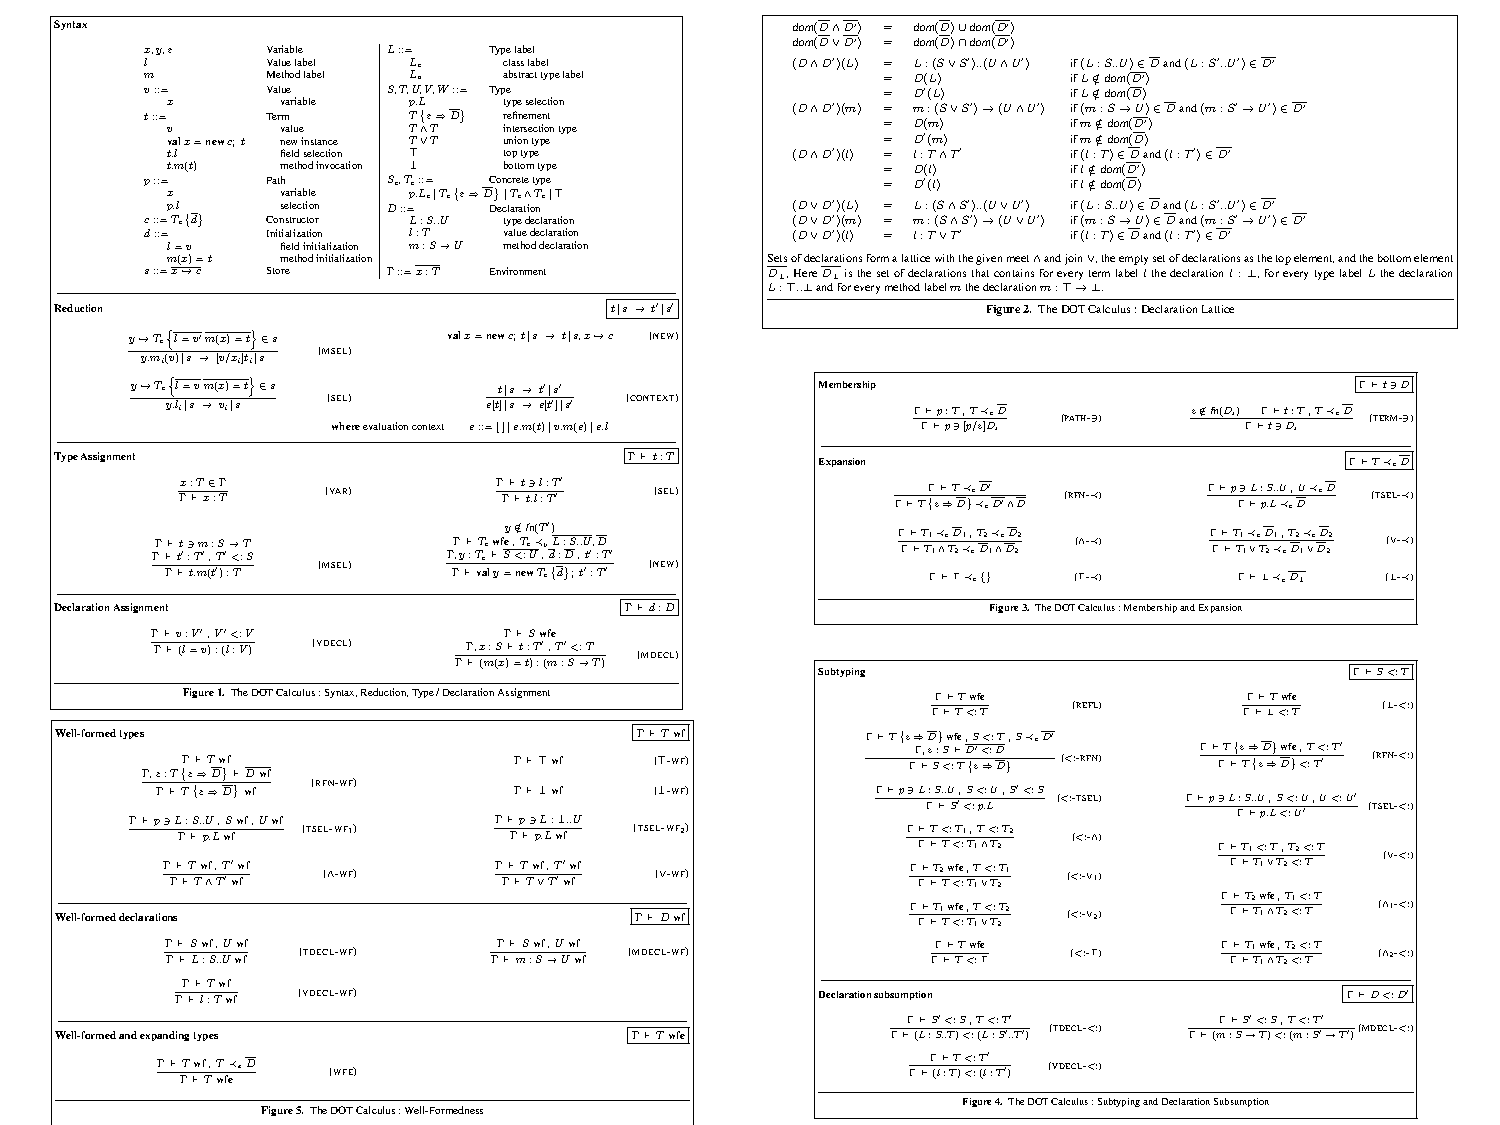
\includegraphics[width=13cm]{fool.pdf}
\end{frame}


\begin{frame}[fragile]{What worked:}
\begin{itemize}
\item Bottom up instead of top down
\item Focus on the core: \\
path-dependent types and objects with (recursive) type members
%\item Mechanized soundness proof!
%\item Valuable insights into why extending the system is hard
\item Look beyond rewriting semantics

\end{itemize}
\end{frame}



%%%%%  intro DOT / Scala


\section{Types in Scala}


% \begin{frame}[fragile]{DOT: Dependent Object Types}
% \begin{itemize}
% \item DOT is a core calculus for path-dependent types.
% \item Aim: simplify Scala's type system and make it more regular.
% \end{itemize}
% \end{frame}

\begin{frame}[fragile]{Modules, Objects, Functions}
\begin{lstlisting}
object listModule {
  trait List[Elem] = {
    def head(): Elem
    def tail(): List[Elem]
  }
  def nil() = new List[Nothing] {
    def head() = error()
    def tail() = error()
  }
  def cons[T](hd: T)(tl: List[T]) = new List[T] {
    def head() = hd
    def tail() = tl
  }
}
\end{lstlisting}
\end{frame}

\begin{frame}[fragile]{Types in Scala}
\begin{description}[functional]
\item[`modular']\begin{description}[higher-kinded types]
\item[named type]@scala.collection.BitSet@
\item[compound type]@Channel with Logged@
\item[refined type]@Channel { def close(): Unit } @
\end{description}
\item[`functional']\begin{description}[higher-kinded types]
\item[parameterized type]@List[String]@
\item[existential type]@List[T] forSome { type T }@
\item[higher-kinded type]@List@
\end{description}
\end{description}
\begin{comment}
too many orthogonal concepts?
can we simplify by keeping only the modular features?
\end{comment}
\end{frame}



\begin{frame}[fragile]{Reducing Functional to Modular}
\begin{itemize}
\item type parameter to type member\\
@class List[Elem] {} /*vs*/ class List { type Elem }@
\item parameterized type to refined type\\
@List[String] /*vs*/ List { type Elem = String }@
\item existential type?\\
@List[T] forSome { type T } /*vs*/ List@
\item higher-kinded type?\\
@List /*vs*/ List@
\end{itemize}
\end{frame}


\begin{frame}[fragile]{Modules, Objects, Functions}
\begin{lstlisting}
val listModule = new { m =>
  type List = { this =>
    type Elem
    def head(): this.Elem
    def tail(): m.List & { type Elem <: this.Elem }
  }
  def nil() = new { this =>
    type Elem = Nothing
    def head() = error()
    def tail() = error()
  }
  def cons[T](hd:T)(tl:m.List & { type Elem <: T }) = new { this =>
    type Elem <: T
    def head() = hd
    def tail() = tl
  }
}
\end{lstlisting}
\end{frame}

\begin{frame}[fragile]{Nominality by Ascription}
\begin{lstlisting}
type ListAPI = { m =>
  type List <: { this =>
    type Elem
    def head(): this.Elem
    def tail(): m.List & { type Elem <: this.Elem }
  }
  def nil(): List & { type Elem = Bot }
  def cons[T]: T => 
    m.List & { type Elem <: T } => 
      m.List & { type Elem <: T }
}
\end{lstlisting}
\end{frame}


\begin{frame}[fragile]{Types in D2 (inspired by DOT)}
\begin{description}[declarations]
\item[types]@S, T, U@
\begin{description}[path-dependent type]
\item[path-dependent type]@p.L@
\item[recursive self type]@{ z => T }@
\item[intersection]@T & T@
\item[union]@T | T@
\item[top]@Any@
\item[bottom]@Nothing@
\item[type declaration]@type L: S .. U@
\item[field declaration]@val l: U@
\item[method declaration]@def m(x: S): U@
\end{description}
\end{description}
\end{frame}



%%%%% µDOT?

%\section{$\mu$DOT}


% \begin{frame}[fragile]{Types in D2 (inspired by DOT)}

% $\begin{array}{ll}
% x, y, z & \mbox{Variable} \\
% S, U, T ::= & \mbox{Type} \\
% \gap  \tbnd{z}{\seq{T}} & \mbox{Recursive Type} \\
% \gap  x.L & \mbox{Type Selection} \\
% %D ::= & \mbox{Member Declaration}\\
% \gap  \tmem{L}{S}{U} & \mbox{Type Member}\\
% %\gap  \tmemup{L}{U}    & \mbox{Type Member (Upper-Bounded)}
% \gap ...&\\
% \end{array}$

% \end{frame}





\begin{frame}[fragile]%{${\mu}${DOT}$_T$: Semantics of Types}

\begin{multicols}{2}[\judgement{Subtyping}{\fbox{$\Gamma \ts S \sub U$}}]
\end{multicols}

\infrule[\textsc{$\sub$-tsel}]
{\Gamma \ts x: (\tmem{L}{S}{U}) \spcomma S' \sub S}
{\Gamma \ts S' \sub x.L}

\infrule[\textsc{tsel-$\sub$}]
{\Gamma \ts x: (\tmem{L}{S}{U}) \spcomma U \sub U'}
{\Gamma \ts x.L \sub U'}

\infrule[\textsc{rec-$\sub$-rec}]
{\Gamma \envplus{z: T} \ts T \sub T'}
{\Gamma \ts \tbnd{z}{T} \sub \tbnd{z}{T'}}

%\begin{multicols}{2}[\judgement{Subtyping of Declarations}{\fbox{$\Gamma \ts D \sub D'$}}]
%\end{multicols}

\infrule[\textsc{tmem-$\sub$-tmem}]
{\Gamma \ts S' \sub S \spcomma U \sub U'}
{\Gamma \ts (\tmem{L}{S}{U}) \sub (\tmem{L}{S'}{U'})}

\end{frame}


%%%%% Transitivity and Narrowing

% \section{Challenges: Transitivity, Narrowing, Inversion}

% \begin{frame}[fragile]{Transitivity, Narrowing}

% \infrule[\textsc{$\sub$-narrow}]
% {\Gamma^a , (x: U) , \Gamma^b \ts T \sub T'\\
%  \Gamma^a \ts S \sub U}
% {\Gamma^a , (x: S) , \Gamma^b \ts T \sub T'}

% \infrule[\textsc{$\sub$-trans}]
% {\Gamma \ts S \sub T \spcomma T \sub U}
% {\Gamma \ts S \sub U}

% \end{frame}



\section{Challenge: Type Preservation}
\begin{frame}[fragile]{Trouble: Type Preservation}
\begin{minted}{scala}
trait Brand {
  type Hidden
  def pack(x: Int): Hidden
  def unpack(x: Hidden): Int
}
val brand: Brand = new Brand {
  type Hidden = Int
  def pack(x: Int): Hidden = x
  def unpack(x: Hidden): Int = x
}
brand.unpack(brand.pack(7)) // ok
brand.unpack(7) // not ok -- but occurs during reduction!
\end{minted}
% \begin{itemize}
% \item Solution: big-step semantics with step-index
% \item Work with types from the original program instead of re-assigning types to partially evaluated terms
% \end{itemize}
\end{frame}



\begin{frame}[fragile]{Trouble: $\Bot$ and Intersections}
Type $\Bot$ is a subtype of all other types, including @{ type E = Int }@
and @{ type E = String }@.

\vspace{1em}
So if p: $\Bot$ we have Int $<:$ p.E and p.E $<:$ String. 

\vspace{1em}
Transitivity would give us Int $<:$ p.E $<:$ String!

\vspace{1em}
Subtyping lattice collapses.

\vspace{1em}
Adding intersection types is equivalent to bottom (bad bounds!)

\end{frame}


\begin{frame}[fragile]{Key Observation}
\begin{itemize}
\item Bottom types do not occur at runtime!
\item It is enough to have transitivity and narrowing on runtime environments
\item Have a (restrictive) static type system and a (lenient) one during evaluation
\end{itemize}
\end{frame}








%%%%% Fsub static semantics

\section{Definitional Interpreters}


\begin{frame}[fragile]{STLC Static Semantics}
\footnotesize\linespread{0.6}
%\bcprulessavespacetrue


\begin{multicols}{2}
\judgement{Syntax}{}

\medskip

$\ba{lll}
  T &::=& X \ |\ \Top \ |\ T \rightarrow T \\
  t &::=& x \ |\ \lambda x:T.t \ |\ t\ t \\
  \Gamma &::=& \emptyset \ |\ \Gamma,x:T
\ea$

\medskip

\judgement{Subtyping}{\fbox{$\Gamma \ts S \sub U$}}

  \infax[]{\Gamma \ts S \sub \Top}

  \vspace{-7mm}\infrule[]{\Gamma \ts T_1 \sub S_1 \spcomma S_2 \sub T_2}
  {\Gamma \ts S_1 \rightarrow S_2 \sub T_1 \rightarrow T_2}

\columnbreak

\judgement{Type assignment}{\fbox{$\Gamma \ts t : T$}}

  \infrule[]{\Gamma \ni x:T}
  {\Gamma \ts x: T}

  \vspace{-7mm}\infrule[]{\Gamma,x:T_1 \ts t_2: T_2}
  {\Gamma \ts \lambda x:T_1.t_2: T_1 \rightarrow T_2}

  \vspace{-7mm}\infrule[]{\Gamma \ts t_1: T_1 \rightarrow T_2 \spcomma t_2: T_1}
  {\Gamma \ts t_1 t_2: T_2}

  \vspace{-7mm}\infrule[]{\Gamma \ts t: S \spcomma S \sub T}
  {\Gamma \ts t: T}

% \judgement{Value type assignment}{\fbox{$H \ts v : T$}}

%   \infax[]{c: B}

%   \infrule{\Gamma \tS H  \gap \Gamma,x:T_1 \ts t: T_2}
%   {\clos{H,\lambda x:T_1.t}: T_1 \rightarrow T_2}

          
\end{multicols}          
\end{frame}


%%%%% Def Int

\begin{frame}[fragile]{STLC}
\begin{lstlisting}[keywords={}]
Fixpoint eval(n: nat)(env: venv)(t: tm){struct n}: 
option (option vl) :=
  DO n1 <== FUEL n;                            (* totality    *)
  match t with
    | tcst c      => DONE VAL (vcst c)         (* constant    *)
    | tvar x      => DONE (lookup x env)       (* variable    *)
    | tabs y      => DONE VAL (vabs env x ey)  (* lambda      *)
    | tapp ef ex  =>                           (* application *)
      DO vf <== eval n1 env ef;
        DO vx <==  eval n1 env ex;
        match vf with
          | (vabs env2 x ey) =>
            eval n1 ((x,vx)::env2) ey
          | _ => ERROR
        end
  end.
\end{lstlisting}
\end{frame}


\begin{frame}[fragile]{Soundness}

\infrule[]
{\Gamma \ts e: T \gap \Gamma \tS H \gap \text{eval } n\ H\ e = \text{Done } r}
{r = \text{Val } v \gap v: T \gap}

\end{frame}


\begin{frame}[fragile]{F$_{<:}$ Static Semantics}
\footnotesize\linespread{0.6}
%\bcprulessavespacetrue


\begin{multicols}{2}
\judgement{Syntax}{}

\medskip

$\ba{lll}
  X &::=& Y \ |\ Z\\
  T &::=& X \ |\ \Top \ |\ T \rightarrow T \ |\ \forall Z<:T.T^Z\\
  t &::=& x \ |\ \lambda x:T.t \ |\ \Lambda Y<:T.t \ |\ t\ t \ |\ t\ [T]\\
  \Gamma &::=& \emptyset \ |\ \Gamma,x:T \ |\ \Gamma,X<:T
\ea$

\medskip

\judgement{Subtyping}{\fbox{$\Gamma \ts S \sub U$}}

  \infax[]{\Gamma \ts S \sub \Top}

  \vspace{-7mm}\infax[]{\Gamma \ts X \sub X}

  \vspace{-7mm}\infrule[]{\Gamma \ni X<:U \gap \Gamma \ts U \sub T}
  {\Gamma \ts X \sub T}

  \vspace{-7mm}\infrule[]{\Gamma \ts T_1 \sub S_1 \spcomma S_2 \sub T_2}
  {\Gamma \ts S_1 \rightarrow S_2 \sub T_1 \rightarrow T_2}

  \vspace{-7mm}\infrule[]{\Gamma \ts T_1 \sub S_1\\\Gamma,Z<:T_1 \ts S_2^Z \sub T_2^Z}
  {\Gamma \ts \forall Z<:S_1.S_2^Z \sub \forall Z<:T_1.T_2^Z}

\judgement{Type assignment}{\fbox{$\Gamma \ts t : T$}}

  \infrule[]{\Gamma \ni x:T}
  {\Gamma \ts x: T}

  \vspace{-7mm}\infrule[]{\Gamma,x:T_1 \ts t_2: T_2}
  {\Gamma \ts \lambda x:T_1.t_2: T_1 \rightarrow T_2}

  \vspace{-7mm}\infrule[]{\Gamma \ts t_1: T_1 \rightarrow T_2 \spcomma t_2: T_1}
  {\Gamma \ts t_1 t_2: T_2}

  \vspace{-7mm}\infrule[]{\Gamma,Y<:T_1 \ts t_2: T_2^Y}
  {\Gamma \ts \Lambda Y<:T_1.t_2: \forall Z<:T_1.T_2^Z}

  \vspace{-7mm}\infrule[]{\Gamma \ts t_1: \forall Z<:T_{11}.T_{12}^Z \spcomma T_2 \sub T_{11}}
  {\Gamma \ts t_1 [T_2]: T_{12}^{T_2}}

  \vspace{-7mm}\infrule[]{\Gamma \ts t: S \spcomma S \sub T}
  {\Gamma \ts t: T}
          
\end{multicols}          
\end{frame}


\begin{frame}[fragile]{F$_{<:}$ --- ?}
$$  (\Lambda X<:T.t) [T] \longrightarrow t[T/X]$$
\end{frame}

\begin{frame}[fragile]{F$_{<:}$ --- ?}
\begin{lstlisting}[keywords={}]
Fixpoint eval(n: nat)(env: venv)(t: tm){struct n}: 
option (option vl) :=
  DO n1 <== FUEL n;                            (* totality    *)
  match t with
    | tcst c      => DONE VAL (vcst c)         (* constant    *)
    | tvar x      => DONE (lookup x env)       (* variable    *)
    | tabs y      => DONE VAL (vabs env x ey)  (* lambda      *)
    | ttabs y     => DONE VAL (vtabs env x ey) (* forall      *)
    | tapp ef ex  =>                           (* application *)
      DO vf <== eval n1 env ef;
        DO vx <==  eval n1 env ex;
        match vf with
          | (vabs env2 x ey) =>
            eval n1 ((x,vx)::env2) ey
          | _ => ERROR
        end
    | ttapp ef T =>
      DO vf <== eval n1 env ef;
        match vf with
          | (vtabs env2 x ey) => eval n1 env2 (substitute ey x T)
          | _ => ERROR
        end
  end.
\end{lstlisting}
\end{frame}


\begin{frame}[fragile]{F$_{<:}$ --- ?}
\begin{lstlisting}[keywords={}]
Fixpoint eval(n: nat)(env: venv)(t: tm){struct n}: 
option (option vl) :=
  DO n1 <== FUEL n;                            (* totality    *)
  match t with
    | tcst c      => DONE VAL (vcst c)         (* constant    *)
    | tvar x      => DONE (lookup x env)       (* variable    *)
    | tabs y      => DONE VAL (vabs env x ey)  (* lambda      *)
    | ttabs y     => DONE VAL (vtabs env x ey) (* forall      *)
    | tapp ef ex  =>                           (* application *)
      DO vf <== eval n1 env ef;
        DO vx <==  eval n1 env ex;
        match vf with
          | (vabs env2 x ey) =>
            eval n1 ((x,vx)::env2) ey
          | _ => ERROR
        end
    | ttapp ef T =>
      DO vf <== eval n1 env ef;
        match vf with
          | (vtabs env2 x ey) => eval n1 ((x,T)::env2) ey
          | _ => ERROR
        end
  end.
\end{lstlisting}
\end{frame}



\begin{frame}[fragile]{F$_{<:}$}
\begin{lstlisting}[keywords={}]
Fixpoint eval(n: nat)(env: venv)(t: tm){struct n}: 
option (option vl) :=
  DO n1 <== FUEL n;                            (* totality    *)
  match t with
    | tcst c      => DONE VAL (vcst c)         (* constant    *)
    | tvar x      => DONE (lookup x env)       (* variable    *)
    | tabs y      => DONE VAL (vabs env x ey)  (* lambda      *)
    | ttabs y     => DONE VAL (vtabs env x ey) (* forall      *)
    | tapp ef ex  =>                           (* application *)
      DO vf <== eval n1 env ef;
        DO vx <==  eval n1 env ex;
        match vf with
          | (vabs env2 x ey) =>
            eval n1 ((x,vx)::env2) ey
          | _ => ERROR
        end
    | ttapp ef T =>
      DO vf <== eval n1 env ef;
        match vf with
          | (vtabs env2 x ey) => eval n1 ((x,vty env T)::env2) ey
          | _ => ERROR
        end
  end.
\end{lstlisting}
\end{frame}



\begin{frame}[fragile]{F$_{<:}$ Dynamics}
\footnotesize
\begin{multicols}{2}
\judgement{Syntax}{}

\medskip

$\ba{lll}
  v &::=& \clos{H,\lambda x:T.t} \ |\ \clos{H,\Lambda Y<:T.t}\\
  H &::=& \emptyset \ |\ H,x:v \ |\  H,Y=\clos{H,T}\\
  J &::=& \emptyset \ |\ J,Z<:\clos{H,T}
\ea$

\medskip

\judgement{Runtime subtp.}{\fbox{$J \ts H_1\ T_1 \sub H_2\ T_2$}}

  \vspace{-0mm}\infax[]{J \ts H_1\ T \sub H_2\ \Top}

%fun
  \vspace{-7mm}\infrule[]{J \ts H_2\ T_1 \sub H_1\ S_1 \gap J \ts H_1\ S_2 \sub H_2\ T_2}
  {J \ts H_1\ S_1 \rightarrow S_2 \sub H_2\ T_1 \rightarrow T_2}

%all
  \vspace{-7mm}\infrule[]{J \ts H_2\ T_1 \sub H_1\ S_1\\
  J,Z<:\clos{H_2,T_1} \ts H_1\ S_2^Z \sub H_2\ T_2^Z}
  {J \ts H_1\ \forall Z<:S_1.S_2^Z \sub H_2\ \forall Z<:T_1.T_2^Z}

%\vspace{15mm}
\columnbreak

Abstract type variables

%selax
  \vspace{-3mm}\infax[]{J \ts H_1\ Z \sub H_2\ Z}

%sela1
  \vspace{-7mm}\infrule[]{J \ni Z<:\clos{H,U} \gap J \ts H\ U \sub H_2\ T}
  {J \ts H_1\ Z \sub H_2\ T}

Concrete type variables

%selx
  \vspace{-3mm}\infrule[]{H_1 \ni Y_1=\clos{H,T} \gap H_2 \ni Y_2=\clos{H,T}}
  {J \ts H_1\ Y_1 \sub H_2\ Y_2}

%sel1
  \vspace{-7mm}\infrule[]{H_1 \ni Y=\clos{H,U} \gap J \ts H\ U \sub H_2\ T}
  {J \ts H_1\ Y \sub H_2\ T}

%sel2
  \vspace{-7mm}\infrule[]{J \ts H_1\ T \sub H\ L \gap H_2 \ni Y=\clos{H,L}}
  {J \ts H_1\ T \sub H_2\ Y}

Transitivity

  \vspace{-3mm}\infrule[]{J \ts H_1\ T1 \sub H_2\ T2 \gap H_2\ T_2 <: H_3\ T_3}
  {J \ts H_1\ T_1 \sub H_3\ T_3}

\end{multicols}
\end{frame}

\begin{frame}[fragile]{F$_{<:}$ Dynamics}
\footnotesize
\begin{multicols}{2}

 \judgement{Value type assignment}{\fbox{$H \ts v : T$}}

   \vspace{-0mm}\infrule[]{\Gamma \tS H\ \emptyset \gap \Gamma,x:T_1 \ts t: T_2}
   {H \ts \clos{H,\lambda x:T_1.t}: T_1 \rightarrow T_2}

   \vspace{-7mm}\infrule[]{\Gamma \tS H\ \emptyset \gap \Gamma,Y<:T_1 \ts t: T_2^Y}
   {H \ts \clos{H,\Lambda Y<:T_1.t}: \forall Z<:T_1.T_2^Z}

   \vspace{-7mm}\infrule[]{H_1 \ts v: T_1  \gap \emptyset \ts H_1\ T_1 \sub H_2\ T_2}
   {H_2 \ts v: T_2}

\columnbreak
 \judgement{Consistent environments}{\fbox{$\Gamma \tS H\ J$}}

   \vspace{-0mm}\infax[]{\emptyset \tS \emptyset\ \emptyset}

   \vspace{-7mm}\infrule[]{\Gamma \tS H\ J \gap  H \ts v: T}
   {\Gamma,x:T \tS (H,x:v)\ J}

   \vspace{-7mm}\infrule{\Gamma \tS H\ J \gap J \ts H_1\ T_1 \sub H\ T}
   {\Gamma,Y<:T \tS (H,Y=\clos{H_1,T_1})\ J}

   \vspace{-7mm}\infrule{\Gamma \tS H\ J \gap J \ts H_1\ T_1 \sub H\ T}
   {\Gamma,Z<:T \tS H\ (J,Z<:\clos{H_1,T_1})}

          
\end{multicols}
\end{frame}



\begin{frame}[fragile]{Challenge: Transitivity}

% \infrule[\textsc{$\sub$-narrow}]
% {\Gamma^a , (x: U) , \Gamma^b \ts T \sub T'\\
%  \Gamma^a \ts S \sub U}
% {\Gamma^a , (x: S) , \Gamma^b \ts T \sub T'}

% \infrule[\textsc{$\sub$-trans}]
% {\Gamma \ts S \sub T \spcomma T \sub U}
% {\Gamma \ts S \sub U}

\infrule[\textsc{$\sub$-trans}]
{J \ts H_1\ T_1 \sub H\ Y \spcomma J \ts H\ Y \sub H_2\ T_2}
{J \ts H_1\ T_1 \sub H_2\ T_2}

\end{frame}



\begin{frame}[fragile]{Challenge: Transitivity}
\begin{itemize}
%\item Attempt 0: independent proofs -- clearly doesn't work
\item Attempt 1: induction on subtyping derivation\\problem: contravariant positions
\item Attempt 2: induction on middle type in $T_1 \sub T_2 \sub T_3$ (like F$_{\sub}$)\\problem: $T_1 \sub Y \sub T_2$
\item Attempt 3: induction on a well-formedness witness\\problem: cyclicity
\item Attempt 4: add transitivity axiom\\problem: inversion lemma
\item Solution: transitivity axiom plus ``push-back'': eliminate 
uses of axiom after the fact
\end{itemize}
\end{frame}




\begin{frame}[fragile]{F$_{<:}$ Extended to Path-Dependent Types}
\scriptsize
\begin{multicols}{2}


\judgement{Syntax}{}

\medskip

$\ba{lll}
  T &::=& x.\text{Type} \ |\  \Top \ |\ (z:T) \rightarrow T^z \ |\ \{\text{Type}=T\}\\
  t &::=& x \ |\  \lambda x:T.t \ |\ t\ t \ |\ \{\text{Type}=T\}\\
  v &::=& \clos{H,\lambda x:T.t} \ |\ \clos{H,T}\\
  G &::=& \emptyset \ |\ G,x:T\\
  H &::=& \emptyset \ |\ H,x:v\\
  J &::=& \emptyset \ |\ H,z:\clos{H,T}
\ea$

\medskip

\judgement{Subtyping}{\fbox{$\Gamma \ts S \sub U$}}

  \infrule[]{\Gamma \ts T_1 \sub T_2 \gap \Gamma \ts T_2 \sub T_1}
  {\Gamma \ts \{\text{Type}=T_1\}\ \sub\ \{\text{Type}=T_2\}}

  \infrule[]{\Gamma(x) = U \gap \Gamma \ts U \sub \{\text{Type}=T\}}
  {\Gamma \ts x.T \sub T}

%  $\ldots$

\judgement{Runtime Subtp.}{\fbox{$J \ts H_1\ T_1 \sub H_2\ T_2$}}

  \infrule[]{J \ts H_1\ T_1 \sub H_2\ T_2  \gap J\ts H_2\ T_2 \sub H_1\ T_1}
  {J \ts H_1\ \{\text{Type}=T_1\}\ \sub\ H_2\ \{\text{Type}=T_2\}}

  \infrule[]{J(z) = \clos{H,U} \gap J \ts H\ U \sub H_2\ \{\text{Type}=T\}}
  {J \ts H_1\ z.\text{Type} \sub H_2\ T}

  \infrule[]{H_1(x)\!=\!v \;\; \ H\!\ts\!v\!: U \gap J \ts H\ U \sub H_2\ \{\text{Type}=T\}}
  {J \ts H_1\ x.\text{Type} \sub H_2\ T}


\end{multicols}
\end{frame}



\begin{frame}[fragile]{F$_{<:}$ Extended to Path-Dependent Types}
\scriptsize
\begin{multicols}{2}

 \judgement{Type assignment}{\fbox{$\Gamma \ts t : T$}}

   \infax[]{\Gamma \ts \{\text{Type}=T\}: \{\text{Type}=T\}}

   \vspace{-7mm}\infrule[]{\Gamma,x:T_1 \ts t_2: T_2^x}
   {\Gamma \ts \lambda x:T_1.t_2: (z:T_1)\rightarrow T_2^z}

   \vspace{-7mm}\infrule[]{\Gamma \ts t_1: (z:T_1)\rightarrow T_2^z  \spcomma t_2: T_1}
   {\Gamma \ts t_1 t_2: T_2}

\columnbreak

 \judgement{Value type assignment}{\fbox{$H \ts v : T$}}

   \infrule[]{\Gamma \tS H\ \emptyset \gap \Gamma \ts \{\text{Type}=T\}: \{\text{Type}=T\}}
   {H \ts \clos{H,T}: \{\text{Type}=T\}}

   \infrule[]{\Gamma \tS H \emptyset \gap \Gamma,x:T_1 \ts t: T_2^x}
   {H \ts \clos{H,\lambda x:T_1.t}: (z:T_1)\rightarrow T_2^z}


\end{multicols}
\end{frame}


\begin{frame}[fragile]{Further Implemented Extensions}
\begin{itemize}
\item Subtyping lattice (intersections and unions)
\item Objects with multiple type and method members
\item Recursive types @{ x => T }@
\item Key technique: more intricate transitivity pushback
\end{itemize}
\end{frame}






%%%%% The End

\section{Thank you!}

% oopsla14.namin.net




%%%%% Type Inference

\section{Type Inference}

\begin{frame}[fragile]{Type Inference in Scala (Least Upper Bound?)}
\begin{minted}{scala}
trait A { type T <: A }
trait B { type T <: B }
trait C extends A with B { type T <: C }
trait D extends A with B { type T <: D }
// in Scala, lub(C, D) is an infinite sequence
A with B { type T <: A with B { type T <: ... } }

// in Scala REPL
> val o = if (true) (new C{}) else (new D{})
o: A with B{type T <: A with B} = ...
> val o:A with B{type T<:A with B {type T<:A with B}} =
          if (true) (new C{}) else (new D{})
o: A with B{type T <: A with B{type T <: A with B}} = ...
\end{minted}
\end{frame}

\begin{frame}[fragile]{Type Inference in Scala (Working too Hard too Soon?)}
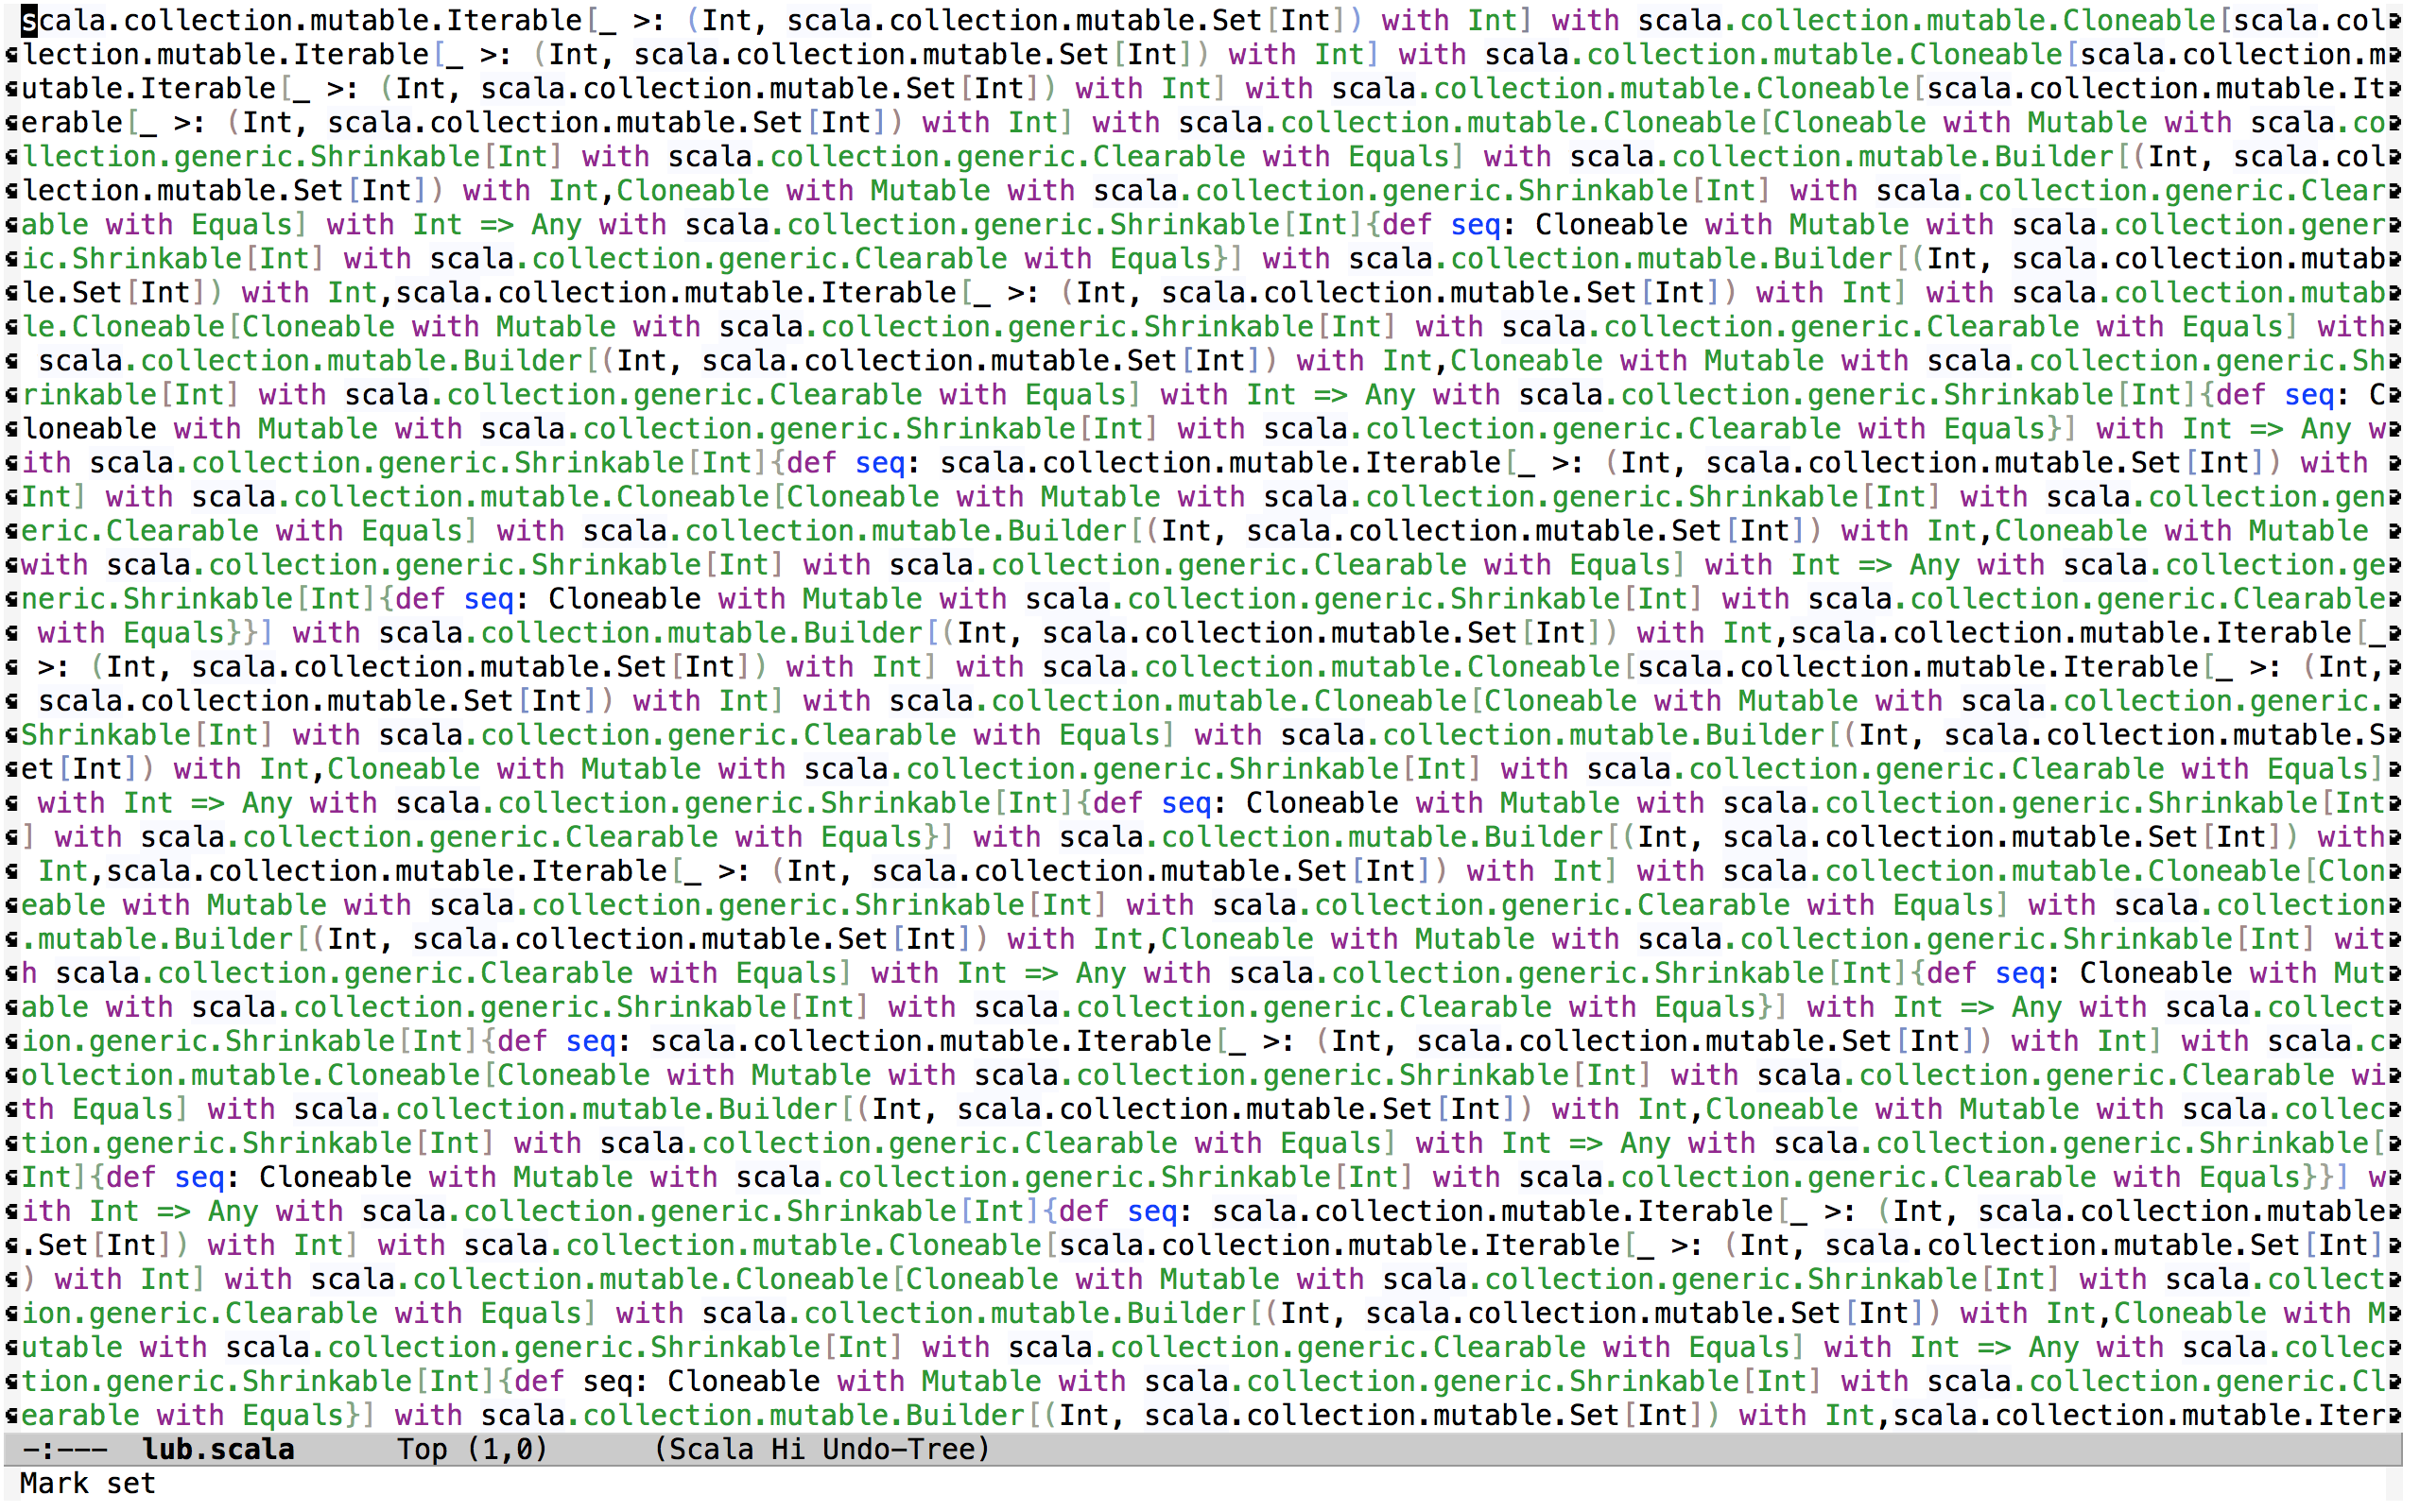
\includegraphics[width=\textwidth]{lub1.png}
\end{frame}

\begin{frame}[fragile]{Type Inference in Scala (Working too Hard too Soon?)}
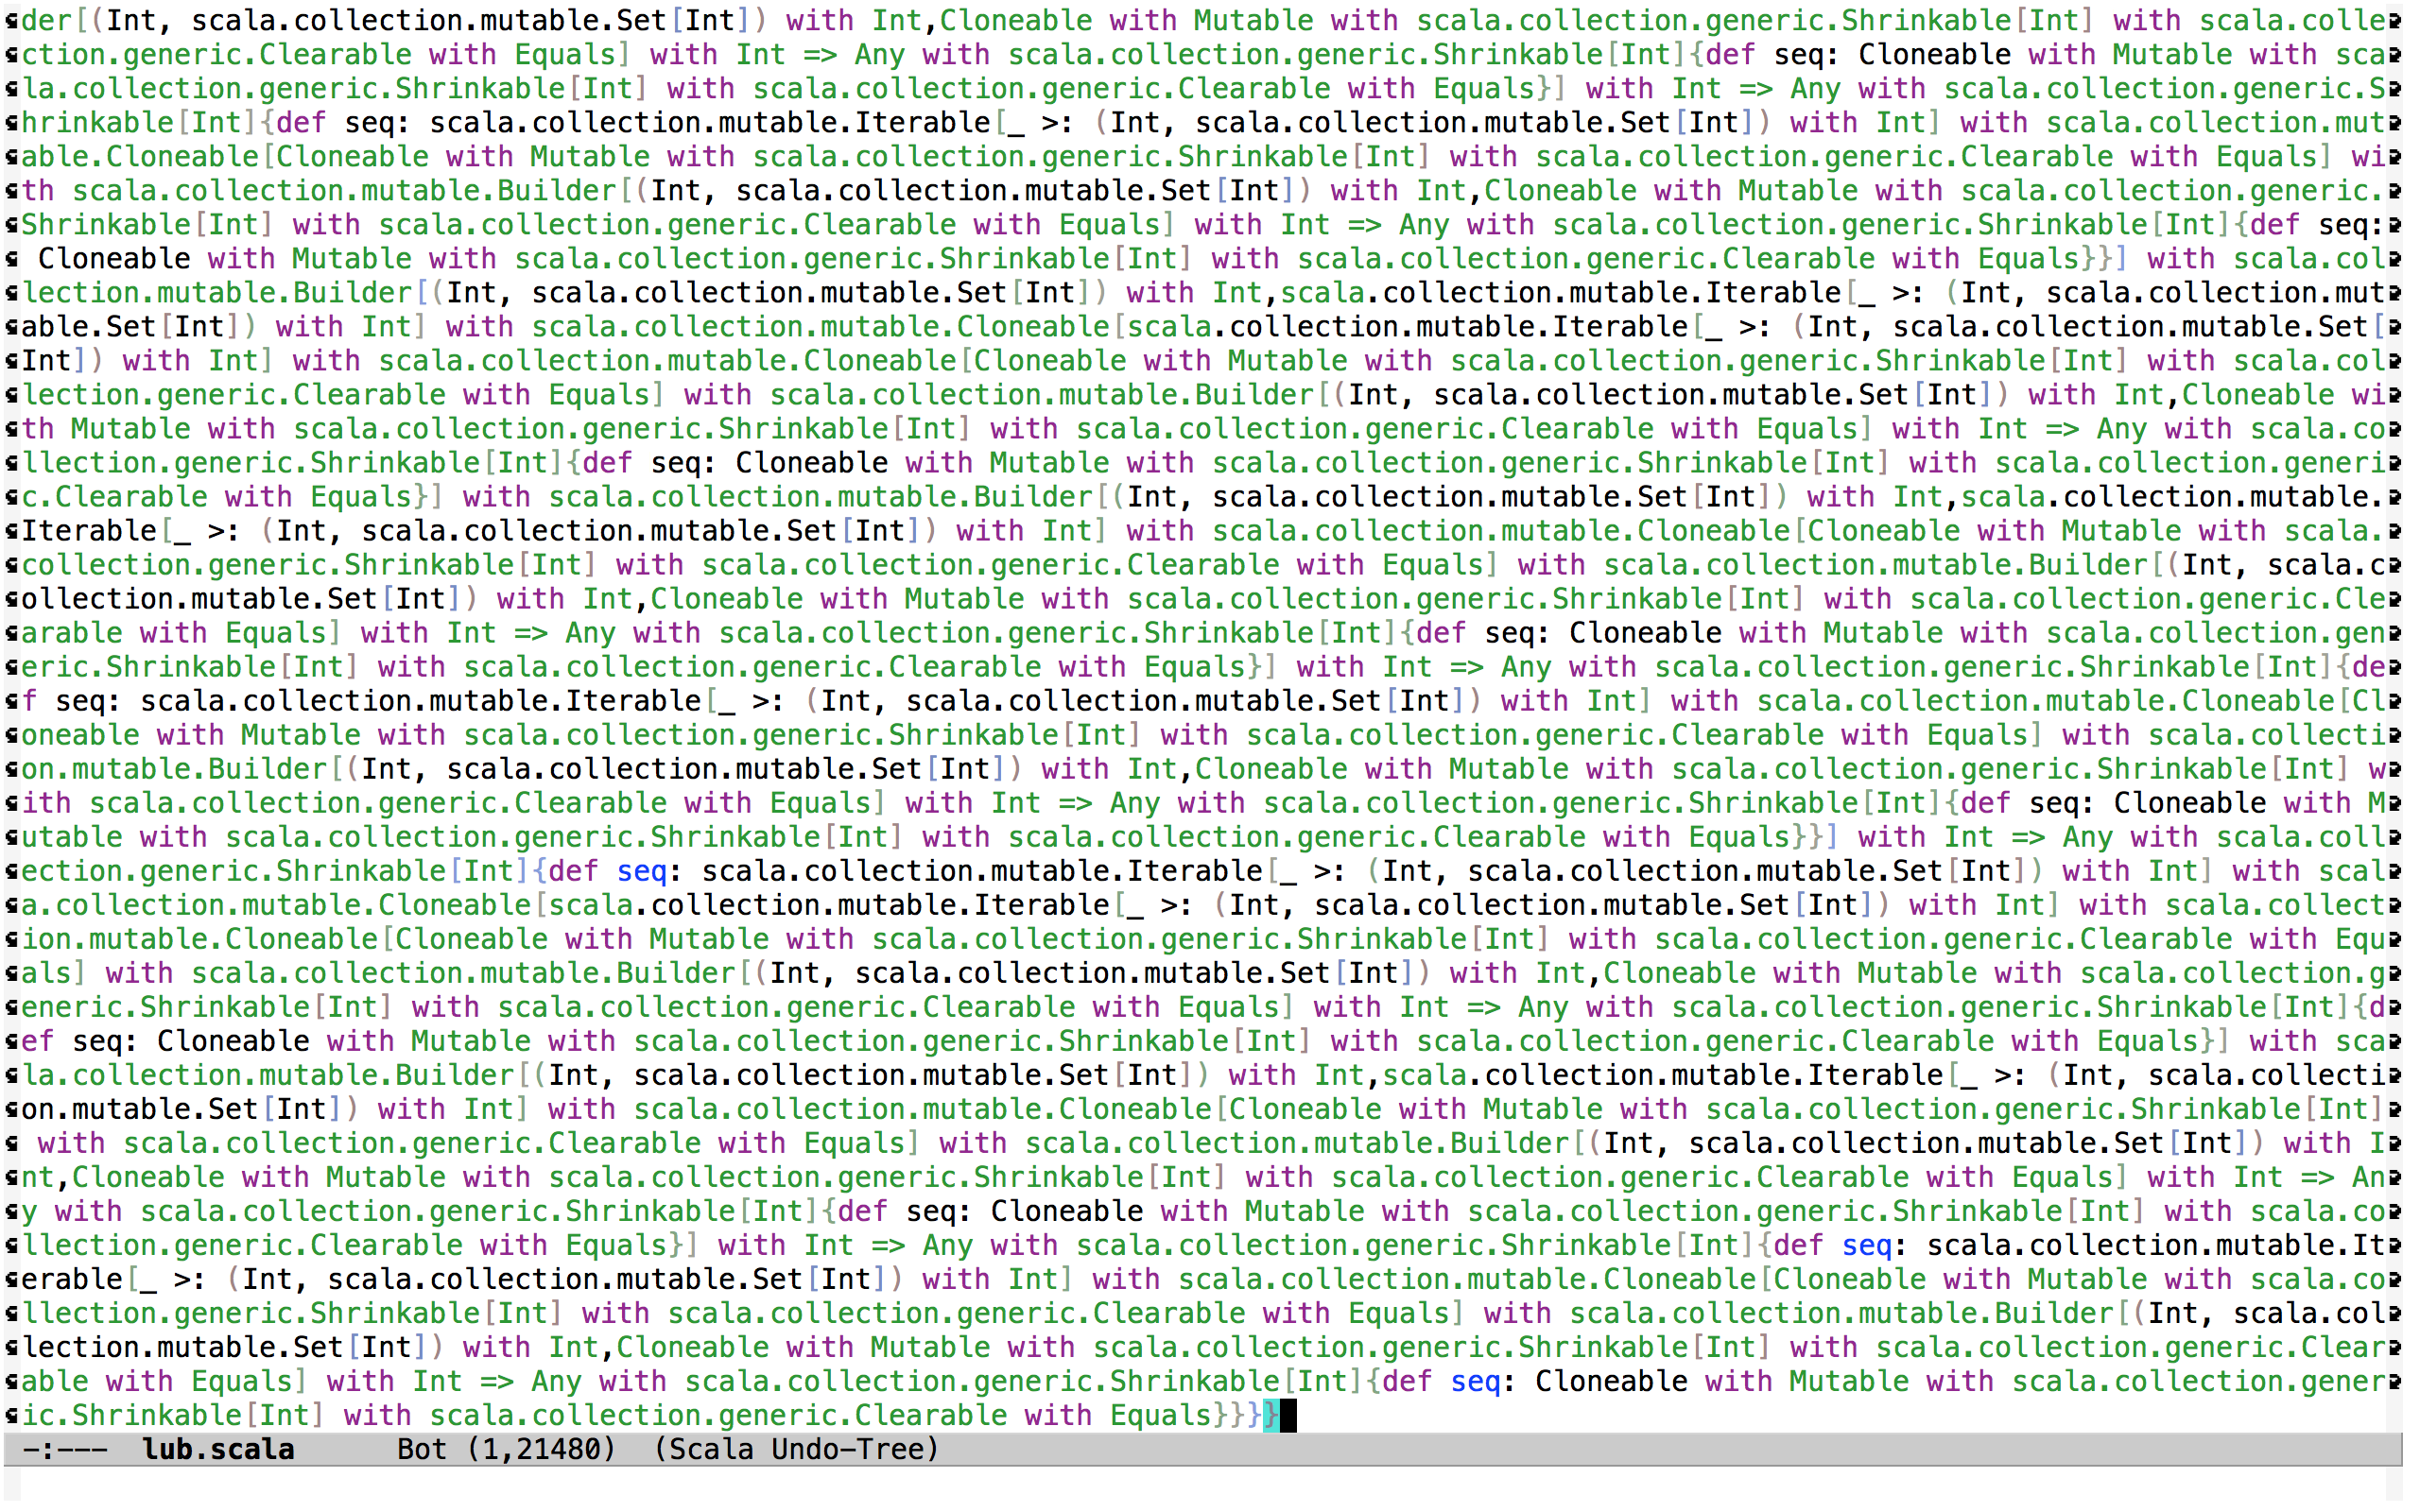
\includegraphics[width=\textwidth]{lub2.png}
\end{frame}

\begin{frame}[fragile]{Type Inference in Scala (Working too Hard too Soon?)}
\begin{minted}{scala}
import scala.collection.mutable.{Map => MMap, Set => MSet}
val ms: MMap[Int, MSet[Int]] = MMap.empty

// in Scala REPL
> if (!ms.contains(1)) ms += 1 -> MSet(1) else ms(1) += 1
res0: ... (796 characters) ...
> :t res0
    : ... (21481 characters) ...
\end{minted}
\begin{itemize}
\item Inspired by a bug report\\
\href{https://issues.scala-lang.org/browse/SI-5862}{SI-5862}: very slow compilation due to humonguous LUB.
\item The character lengths reported are for Scala 2.11 ({\em after} the fix).
\item In Dotty, type inference can be lazy thanks to the native unions (for least upper bounds) and intersections (for greatest lower bounds) of the core calculus (DOT).
\end{itemize}
\end{frame}


\end{document}
